% Provenance (never printed): see sources/outline_sources.md (Year 2: energy geology --- the
% petroleum system quantified, unconventional resources, geothermal systems, uranium deposits,
% geological storage of carbon dioxide).
% Kerogen kinetics and elemental analyses: Fletcher and Pugmire (DOE, OSTI 1176871); kerogen
% types and Easy%Ro: Advanced Chemistry Basins Project (DOE, OSTI 830009); maturity thresholds:
% USGS MF-2008-B; TTI: Waples (1980) and Hammerschmidt et al. (2014); volumetrics and CO2
% storage: DOE/NETL (2008) and IPCC SRCCS (2005) chapter 5; geothermal: USGS OFR 2008-1296 and
% FS 2008-3082; uranium: USGS Bulletin 1693; Oklo: OSTI abstract records. Ledger rows in
% sources/ledger/book4.md; curves from figdata/bachelor-2/maturation.py and co2_density.py,
% numbers from the Book 4 second-writer scratch calculator calc/ch30.py.
% Geology and sourced numbers only: no advocacy, no policy.
\chapter{Géologie énergétique}\label{ch:b2:energy-geology}

Le pétrole résulte des restes d'organismes microscopiques, enfouis avec la boue et cuits pendant des millions d'années
vers \qty{100}{\celsius}~; la géothermie est la même chaleur de la Terre, prélevée directement.
Les deux sont gouvernées par la température et par le temps~: la première par la vitesse à laquelle une réaction chimique se déroule
à mesure que les roches enfouies se réchauffent lentement, la seconde par la quantité de chaleur qu'un volume de roche emmagasine
et par la vitesse à laquelle l'eau peut la transporter jusqu'à un puits. Ce chapitre quantifie le système pétrolier et examine les ressources
qui manquent de l'un de ses éléments, puis la chaleur géothermique et l'uranium,
et se termine par l'opération inverse~: remettre le dioxyde de carbone dans le sous-sol.
% ledger: earle:oil-window, earle:organic-preservation

\begin{recall}
\textbf{Des volumes scolaires}~: roche mère, kérogène, maturation, fenêtre à huile, migration, roche réservoir, couverture, piège,
charge sédimentaire, système pétrolier~; houille et rang du charbon~; énergie géothermique. \textbf{Du volume de première année}~: flux de chaleur
et géotherme~; porosité et perméabilité~; pression du fluide interstitiel, contrainte effective et critère de Coulomb~; diagraphie~;
bassin sédimentaire et subsidence. \textbf{Des volumes de chimie}~: la loi d'Arrhenius, l'énergie d'activation, la réaction d'ordre un.
\textbf{Des volumes de physique}~: la désintégration radioactive, la constante de désintégration, la demi-vie~;
le point critique d'un fluide.
\textbf{Du \cref{ch:b2:basins-compared}}~: \omterm{def:b2:basins-compared:curve}{courbe de subsidence}.
\textbf{Du \cref{ch:b2:ore-deposits}}~: \omterm{def:b2:ore-deposits:types}{type de gisement}, \omterm{def:b2:ore-deposits:grade}{tonnage}.
\end{recall}

\section{Le système pétrolier quantifié}\label{sec:b2:energy-geology:petroleum}

Un système pétrolier exige une roche mère riche en kérogène, un réservoir, une couverture, un piège
et une charge sédimentaire suffisante pour réchauffer la roche mère, et ses événements doivent se succéder dans le bon ordre~:
le piège doit exister au moment où l'huile migre. Le quantifier revient à répondre à trois questions~: quel type de kérogène
contient la roche mère, jusqu'à quel point ce kérogène a été transformé, et quelle part du produit
se trouve dans le piège.
% ledger: magoon00:tps

\begin{definition}[Type de kérogène, diagramme de van Krevelen]\label{def:b2:energy-geology:kerogen}
Les kérogènes se répartissent en trois \emph{types de kérogène}\index{types de kérogène} selon leur composition élémentaire~:
type~I, sapropélique, le plus riche en hydrogène, qui engendre surtout de l'huile~; type~III, humique ou charbonneux,
pauvre en hydrogène, qui engendre surtout du méthane~; et type~II, intermédiaire, source d'huile et de gaz à la fois.
Le \emph{diagramme de van Krevelen}\index{diagramme de van Krevelen} trace le rapport atomique H/C d'un kérogène en fonction de son rapport atomique O/C~;
les types occupent des régions différentes du diagramme, et la maturation
déplace un kérogène vers les faibles H/C et les faibles O/C.
\end{definition}

Sept kérogènes immatures de type connu, analysés dans un même laboratoire, ont un H/C atomique
de 1.51 et 1.61 (type~I, parmi eux le schiste bitumineux de Green River dans l'Utah, déposé dans des lacs et riche en restes d'algues),
de 1.22 à 1.28 (type~II, parmi eux l'argile de Kimmeridge de la mer du Nord), de 1.13 (un mélange de type~II/III) et de 0.99 (type~III, le charbon de Cameo dans le Colorado).
Le kérogène de Green River, à \qty{77}{\percent} de carbone en masse, a pour moyenne C$_{100}$H$_{150}$N$_3$O$_8$S~: H/C 1.50 et
O/C 0.08. Chauffé en laboratoire à \qty{10}{K} par minute, il laisse un résidu dont le H/C tombe à
1.20 à \qty{460}{\celsius} puis à 0.54 à \qty{525}{\celsius},
tandis que son O/C passe de 0.08 à environ
0.01~: le chemin tracé à gauche de la figure ci-dessous.
% ledger: acb04:kerogens, fp14:gr-kerogen, fp14:gr-chars, mf88:thresholds
% values: GR3.9 kerogen H/C 1.486, O/C 0.080; chars 460 C 1.200/0.016, 525 C 0.544/0.011 (figdata maturation.py vk)

\begin{omfigure}
\centering
\begin{minipage}[b]{0.49\linewidth}\centering
\begin{tikzpicture}
\begin{axis}[omrecord, width=0.95\linewidth, height=5.0cm, xmin=0, xmax=0.12, ymin=0, ymax=1.8,
  xlabel={rapport atomique O/C}, ylabel={rapport atomique H/C}, xtick={0,0.04,0.08}, scaled x ticks=false,
  xticklabel style={/pgf/number format/fixed}, tick label style={font=\scriptsize},
  label style={font=\small}]
% computed in figdata/bachelor-2/maturation.py part vk; ledger: fp14:gr-kerogen, fp14:gr-chars
\addplot[omThm, line width=0.9pt, mark=*, mark size=1.3pt, -{Stealth[length=4pt]}] table[x=oc, y=hc] {figdata/out/bachelor-2-maturation-vk.dat};
\node[font=\scriptsize, text=omThm, anchor=north east] at (axis cs:0.081,1.45) {kérogène};
\node[font=\scriptsize, text=omThm, anchor=west] at (axis cs:0.013,0.52) {\qty{525}{\celsius}};
% ledger: acb04:kerogens (H/C of immature kerogens; O/C not reported)
\draw[omThm, line width=1pt] (axis cs:0.104,1.51) -- (axis cs:0.12,1.51);
\draw[omThm, line width=1pt] (axis cs:0.104,1.61) -- (axis cs:0.12,1.61);
\draw[omProp, line width=1pt] (axis cs:0.104,1.22) -- (axis cs:0.12,1.22);
\draw[omProp, line width=1pt] (axis cs:0.104,1.25) -- (axis cs:0.12,1.25);
\draw[omProp, line width=1pt] (axis cs:0.104,1.28) -- (axis cs:0.12,1.28);
\draw[omExo, line width=1pt] (axis cs:0.104,1.13) -- (axis cs:0.12,1.13);
\draw[omDef, line width=1pt] (axis cs:0.104,0.99) -- (axis cs:0.12,0.99);
\node[font=\scriptsize, text=omThm, anchor=east] at (axis cs:0.103,1.58) {I};
\node[font=\scriptsize, text=omProp, anchor=east] at (axis cs:0.103,1.25) {II};
\node[font=\scriptsize, text=omDef, anchor=east] at (axis cs:0.103,0.97) {III};
\end{axis}
\end{tikzpicture}
\end{minipage}\hfill
\begin{minipage}[b]{0.49\linewidth}\centering
\begin{tikzpicture}
\begin{axis}[omrecord, width=0.95\linewidth, height=5.0cm, xmin=60, xmax=220, ymin=0, ymax=1,
  xlabel={température (\unit{\celsius})}, ylabel={taux de transformation},
  tick label style={font=\scriptsize}, label style={font=\small}]
% computed in figdata/bachelor-2/maturation.py part tr; ledger: fp14:gr-daem
\addplot[black!40, densely dotted] coordinates {(60,0.5) (220,0.5)};
\addplot[omDef, line width=1.1pt] table[x=t_c, y=tr1] {figdata/out/bachelor-2-maturation-tr.dat};
\addplot[omThm, line width=1.1pt] table[x=t_c, y=tr10] {figdata/out/bachelor-2-maturation-tr.dat};
\addplot[omDef, line width=0.6pt, densely dashed] table[x=t_c, y=app1] {figdata/out/bachelor-2-maturation-tr.dat};
\addplot[omThm, line width=0.6pt, densely dashed] table[x=t_c, y=app10] {figdata/out/bachelor-2-maturation-tr.dat};
\node[font=\scriptsize, text=omDef, anchor=east] at (axis cs:125,0.80) {\qty{1}{\celsius\per\Ma}};
\node[font=\scriptsize, text=omThm, anchor=west] at (axis cs:160,0.30) {\qty{10}{\celsius\per\Ma}};
\end{axis}
\end{tikzpicture}
\end{minipage}
\par\smallskip{\small À gauche~: un \omterm{def:b2:energy-geology:kerogen}{diagramme de van Krevelen}. Le trajet rouge est celui du kérogène de Green River de type~I
et de ses résidus après chauffage en laboratoire à \qty{10}{K} par minute de 400 à \qty{525}{\celsius}~; les traits
à droite marquent le H/C de sept kérogènes immatures de type~I (rouge), II (orange),
II/III (gris) et III (bleu), dont le O/C n'était pas indiqué. Données~: Fletcher et Pugmire (2014)~; Advanced Chemistry Basins Project (2004).
À droite~: taux de transformation du kérogène
de Green River chauffé à vitesse constante à partir de \qty{10}{\celsius}, avec sa distribution d'énergies d'activation (trait plein)
et avec son énergie moyenne seule, par \eqref{eq:b2:energy-geology:maturation} (tirets).}
\end{omfigure}

La conversion du kérogène en pétrole est un ensemble de réactions d'ordre un, obéissant chacune à la loi
d'Arrhenius. Dans un bassin en subsidence, la température d'une roche mère s'élève lentement et presque régulièrement, ce qui fait du résultat suivant
le cœur des modèles de maturation.

\begin{proposition}[Réaction d'ordre un à vitesse de chauffe constante]\label{prop:b2:energy-geology:maturation}
Soit une réaction d'ordre un de constante de vitesse $k = A\,e^{-E/RT}$ se déroulant dans un matériau chauffé à
la vitesse constante $\beta = \mathrm{d}T/\mathrm{d}t$ à partir d'une température $T_0$ à laquelle $k$ est négligeable.
La fraction non convertie à la température $T$ vaut
\begin{equation}
x(T) = \exp\Bigl[-\frac{A}{\beta}\int_{T_0}^{T} e^{-E/RT'}\,\mathrm{d}T'\Bigr]
\approx \exp\Bigl[-\frac{A R T^2}{\beta E}\,e^{-E/RT}\Bigr] ,
\label{eq:b2:energy-geology:maturation}
\end{equation}
l'approximation étant valable lorsque $E/RT \gg 1$~; le taux de transformation est $1 - x$.
\end{proposition}

\begin{proof}
L'ordre un signifie $\mathrm{d}x/\mathrm{d}t = -k x$. Avec $\mathrm{d}t = \mathrm{d}T/\beta$,
$\mathrm{d}\ln x = -(A/\beta)\,e^{-E/RT}\,\mathrm{d}T$, et l'intégration à partir de $x = 1$ en $T_0$ donne
la première forme. Pour l'intégrale, $\frac{\mathrm{d}}{\mathrm{d}T}\bigl[\frac{RT^2}{E}e^{-E/RT}\bigr]
= \bigl(1 + \frac{2RT}{E}\bigr)e^{-E/RT}$, donc l'intégrale vaut $\frac{RT^2}{E}e^{-E/RT}$ à une
correction relative d'ordre $2RT/E$ près, la borne inférieure ne contribuant rien car $e^{-E/RT_0} \ll
e^{-E/RT}$.
\end{proof}

Deux conséquences en découlent. La conversion se produit sur un intervalle étroit de températures, car
$e^{-E/RT}$ varie si vite (exercice~\ref{exo:b2:energy-geology:11}). Un chauffage plus lent convertit
à plus basse température~: en prenant $x = 1/2$, une vitesse de chauffe dix fois plus rapide élève la température de demi-conversion
d'environ $(RT^2/E)\ln 10$. La cinétique du kérogène de Green River, ajustée sur des pyrolyses de laboratoire, donne $A = \qty{9.21e13}{s^{-1}}$ et $E/R = \qty{26800}{K}$ ($E =
\qty{223}{kJ/mol}$)~; avec cette énergie unique, la demi-conversion survient à \qty{136.4}{\celsius} pour \qty{1}{\celsius\per\Ma}
et à \qty{150.9}{\celsius} pour \qty{10}{\celsius\per\Ma}, soit un décalage de
\qty{14.5}{\celsius} contre $6.26 \times \ln 10 = \qty{14.4}{K}$ prévu. Chauffé à
\qty{10}{K} par minute, le même kérogène se convertit vers \qty{450}{\celsius}
(exercice~\ref{exo:b2:energy-geology:6})~: le temps tient lieu de température. C'est pourquoi la cinétique se mesure par pyrolyse
vers 250 à \qty{600}{\celsius}, et pourquoi extrapoler ces lois sur douze ordres de grandeur
de vitesse de chauffe laisse incertaine
la profondeur prévue de la fenêtre à huile.
% ledger: fp14:gr-daem, acb04:kinetic-spread, codata:R
% values: Thalf 136.403 / 150.873 C; RT2/E 6.2587 K; lab 445.9 C (figdata maturation.py numbers, calc/ch30.py)

Un kérogène réel possède des liaisons de forces très diverses~: sa cinétique est donc une distribution d'énergies d'activation, chaque fraction
obéissant à la proposition~; pour le kérogène de Green River, la distribution est normale,
avec un écart type $\sigma/R = \qty{481}{K}$.
La distribution élargit la conversion, comme le montre le côté droit de la figure~: à \qty{150}{\celsius}, le kérogène chauffé à
\qty{1}{\celsius\per\Ma} est converti à \qty{93}{\percent}, celui chauffé dix fois plus vite
à \qty{48}{\percent}.
% ledger: fp14:gr-daem
% values: TR 0.927 / 0.484 at 150 C (figdata maturation.py numbers)

\begin{definition}[Réflectance de la vitrinite, indice temps--température]\label{def:b2:energy-geology:maturity}
\emph{Réflectance de la vitrinite}\index{réflectance de la vitrinite}, $R_o$, est le pourcentage de la lumière incidente
réfléchie par des grains polis de vitrinite, un constituant organique du charbon et du kérogène,
mesuré au microscope~; elle croît de façon irréversible avec le chauffage et enregistre la maturité thermique la plus élevée qu'une roche ait atteinte. Le
\emph{indice temps--température}\index{indice temps--température} (TTI) de Lopatin est la somme
$\sum_n \Delta t_n\,2^n$ sur les intervalles de \qty{10}{\celsius} que la roche a traversés,
$\Delta t_n$ étant le temps, en millions d'années, passé dans l'intervalle numéroté $n$, avec $n = 0$
pour 100 à \qty{110}{\celsius}, $n = 1$ pour 110 à \qty{120}{\celsius}, $n = -1$ pour 90 à
\qty{100}{\celsius}, et ainsi de suite.
\end{definition}

Sur l'échelle de réflectance, la génération d'huile à partir des kérogènes de types I et II commence près de $R_o =
\qty{0.60}{\percent}$~; au-delà de 1.20 à \qty{1.30}{\percent}, l'huile n'est plus stable et se décompose en
méthane~; le type~III commence à produire du méthane vers \qty{0.73}{\percent}, et la génération de gaz se poursuit jusqu'à
environ \qty{4.8}{\percent}. Les modèles calculent $R_o$ comme un kérogène~: le modèle Easy\%Ro
traite la vitrinite comme vingt réactions parallèles d'ordre un de $A = \qty{e13}{s^{-1}}$ et d'énergies
comprises entre 34 et \qty{72}{kcal/mol} (142 à \qty{301}{kJ/mol}), et transforme leur fraction convertie $F$,
d'au plus 0.85, en $R_o = \exp(-1.6 + 3.7F)$, qui varie de 0.20 à \qty{4.7}{\percent}.
% ledger: mf88:thresholds, acb04:easyro, fp14:gr-chars

La réflectance se calcule de la même façon le long de chaque horizon d'un bassin. Dans le bassin fictif de la figure
ci-dessous, les sédiments se sont accumulés à \qty{100}{m} par million d'années de 100 à \qty{70}{\Ma},
puis à \qty{35}{m} par million d'années, sous une surface à \qty{10}{\celsius} et avec un gradient stable de
\qty{30}{\celsius\per\km}. Son horizon le plus ancien a atteint $R_o = \qty{0.6}{\percent}$ à
\qty{67.6}{\Ma}, à \qty{3080}{m} et \qty{102}{\celsius}, et \qty{1.3}{\percent} à
\qty{11.6}{\Ma}, à \qty{5040}{m} et \qty{161}{\celsius}~; il se trouve aujourd'hui à \qty{5450}{m} et
\qty{173.5}{\celsius}, avec $R_o = \qty{1.54}{\percent}$. Le géotherme étant stable, les
fronts de réflectance suivent presque les isothermes, le début de la génération d'huile vers
\qty{100}{\celsius}, dans les 60 à \qty{120}{\celsius} des volumes scolaires.
% ledger: acb04:easyro, mf88:thresholds, earle:settings, earle:oil-window
% values: figdata maturation.py numbers (oldest_ro06_*, oldest_ro13_*, ro_oldest_now)

\begin{omfigure}
\centering
\begin{tikzpicture}
\begin{axis}[omrecord, width=0.86\linewidth, height=4.8cm, xmin=0, xmax=100, ymin=0, ymax=5.6,
  x dir=reverse, y dir=reverse, ylabel={profondeur (km)}, xticklabels={}, name=bh,
  tick label style={font=\scriptsize}, label style={font=\small}]
% computed in figdata/bachelor-2/maturation.py parts burial and fronts (invented basin)
\addplot[black!40, densely dashed] coordinates {(100,1.333) (0,1.333)};
\addplot[black!40, densely dashed] coordinates {(100,3.0) (0,3.0)};
\addplot[black!40, densely dashed] coordinates {(100,4.667) (0,4.667)};
\node[font=\tiny, text=black!60, anchor=south east, fill=white, inner sep=1pt] at (axis cs:1,1.333) {\qty{50}{\celsius}};
\node[font=\tiny, text=black!60, anchor=south east, fill=white, inner sep=1pt] at (axis cs:1,3.0) {\qty{100}{\celsius}};
\node[font=\tiny, text=black!60, anchor=south east, fill=white, inner sep=1pt] at (axis cs:1,4.667) {\qty{150}{\celsius}};
\addplot[black!70, line width=0.5pt, unbounded coords=jump] table[x=t_ma, y expr=\thisrow{d90}/1000] {figdata/out/bachelor-2-maturation-burial.dat};
\addplot[black!70, line width=0.5pt, unbounded coords=jump] table[x=t_ma, y expr=\thisrow{d80}/1000] {figdata/out/bachelor-2-maturation-burial.dat};
\addplot[black!70, line width=0.5pt, unbounded coords=jump] table[x=t_ma, y expr=\thisrow{d70}/1000] {figdata/out/bachelor-2-maturation-burial.dat};
\addplot[black!70, line width=0.5pt, unbounded coords=jump] table[x=t_ma, y expr=\thisrow{d60}/1000] {figdata/out/bachelor-2-maturation-burial.dat};
\addplot[black!70, line width=0.5pt, unbounded coords=jump] table[x=t_ma, y expr=\thisrow{d50}/1000] {figdata/out/bachelor-2-maturation-burial.dat};
\addplot[black!70, line width=0.5pt, unbounded coords=jump] table[x=t_ma, y expr=\thisrow{d40}/1000] {figdata/out/bachelor-2-maturation-burial.dat};
\addplot[black!70, line width=0.5pt, unbounded coords=jump] table[x=t_ma, y expr=\thisrow{d30}/1000] {figdata/out/bachelor-2-maturation-burial.dat};
\addplot[black!70, line width=0.5pt, unbounded coords=jump] table[x=t_ma, y expr=\thisrow{d20}/1000] {figdata/out/bachelor-2-maturation-burial.dat};
\addplot[black!70, line width=0.5pt, unbounded coords=jump] table[x=t_ma, y expr=\thisrow{d10}/1000] {figdata/out/bachelor-2-maturation-burial.dat};
\addplot[black, line width=1.1pt, unbounded coords=jump] table[x=t_ma, y expr=\thisrow{d100}/1000] {figdata/out/bachelor-2-maturation-burial.dat};
\addplot[omDef, line width=1.4pt, unbounded coords=jump] table[x=t_ma, y expr=\thisrow{z06}/1000] {figdata/out/bachelor-2-maturation-fronts.dat};
\addplot[omThm, line width=1.4pt, unbounded coords=jump] table[x=t_ma, y expr=\thisrow{z13}/1000] {figdata/out/bachelor-2-maturation-fronts.dat};
\node[font=\scriptsize, text=omDef, anchor=north, fill=white, inner sep=1pt] at (axis cs:40,3.05) {$R_o = \qty{0.6}{\percent}$};
\node[font=\scriptsize, text=omThm, anchor=north west, fill=white, inner sep=1pt] at (axis cs:9,5.10) {\qty{1.3}{\percent}};
\node[font=\scriptsize, anchor=north east, fill=white, inner sep=1pt] at (axis cs:58,4.75) {roche mère};
\end{axis}
\begin{axis}[at={(bh.south west)}, anchor=north west, yshift=-0.15cm, width=0.86\linewidth,
  height=2.9cm, xmin=0, xmax=100, ymin=0.4, ymax=6.6, x dir=reverse, y dir=reverse,
  xlabel={temps (\unit{\Ma})}, ytick={1,2,3,4,5,6},
  yticklabels={roche mère, roche réservoir, roche de couverture, charge sédimentaire, formation piège, génération},
  tick label style={font=\tiny}, label style={font=\small}, axis line style={black!60},
  xtick={100,80,60,40,20,0}]
% schematic events chart of the same invented basin
\fill[omLithShale!80!black] (axis cs:100,0.75) rectangle (axis cs:96,1.25);
\fill[omLithSand!70!black] (axis cs:90,1.75) rectangle (axis cs:85,2.25);
\fill[omLithShale!80!black] (axis cs:85,2.75) rectangle (axis cs:80,3.25);
\fill[black!25] (axis cs:80,3.75) rectangle (axis cs:0,4.25);
\fill[omProp!70] (axis cs:75,4.75) rectangle (axis cs:70,5.25);
\fill[omDef!70] (axis cs:67.6,5.75) rectangle (axis cs:11.6,6.25);
\end{axis}
\end{tikzpicture}
\par\smallskip{\small En haut~: histoire d'enfouissement d'un bassin fictif (noir~: horizons déposés tous les
10 millions d'années, le plus épais étant la roche mère), isothermes (tirets) et profondeurs où
Easy\%Ro atteint \qty{0.6}{\percent} (bleu) et \qty{1.3}{\percent} (rouge). En bas~: son diagramme d'événements~;
la génération va de $R_o = \qty{0.6}{\percent}$ à \qty{1.3}{\percent} dans la roche mère,
après la formation du piège.}
\end{omfigure}

La TTI est plus ancienne et plus grossière. Elle suppose que la maturation double sa vitesse pour chaque hausse de
\qty{10}{\celsius}, comme le fait près de \qty{100}{\celsius} une loi d'Arrhenius d'énergie $E \approx \qty{82}{kJ/mol}$
(exercice~\ref{exo:b2:energy-geology:5})~; sur son échelle, Waples plaça le début de la génération d'huile
à une TTI de 15, son maximum à 75 et sa fin à 160.
% ledger: waples80:tti, hamm14:tti-table

\begin{method}[Calcul d'un indice temps--température]\label{met:b2:energy-geology:tti}
Les données sont l'histoire d'enfouissement de la roche mère et le géotherme, supposé stable.
\begin{enumerate}
  \item \textbf{Trajet thermique.} Convertir la profondeur en température à chaque instant~: température de surface
        plus gradient multiplié par la profondeur.
  \item \textbf{Temps dans les intervalles.} Trouver le temps $\Delta t_n$ passé dans chaque intervalle de
        \qty{10}{\celsius}~; si la vitesse de chauffe $\beta$ est constante, $\Delta t_n = \qty{10}{\celsius}/\beta$.
  \item \textbf{Somme.} Additionner les produits $\Delta t_n\,2^n$ dans l'ordre du temps~; le début, le maximum
        et la fin de la génération d'huile sont atteints lorsque la somme cumulée passe par 15, 75 et 160.
\end{enumerate}
\end{method}

Les modèles de bassin expriment la conversion par un taux de transformation~: la fraction du potentiel
d'hydrocarbures initial d'une roche mère déjà convertie. Dans un modèle d'un bassin californien, l'expulsion
depuis la roche mère était supposée commencer à un taux de \qty{10}{\percent}, culminer à \qty{50}{\percent}
et s'achever à \qty{95}{\percent}. L'huile expulsée, plus légère que l'eau,
migre vers le haut dans des roches réservoirs perméables et y est retenue là où une couverture ferme un piège.
% ledger: peters08b4:tr, magoon00:tps, earle:migration-traps

\begin{proposition}[Pétrole en place]\label{prop:b2:energy-geology:volumetrics}
Soit un piège d'aire $A$ et un réservoir d'épaisseur utile $h$, de porosité $\phi$ et de saturation en eau
$S_w$, et soit $B_o$ le facteur volumique de formation de son huile, c'est-à-dire le rapport du volume qu'une quantité
d'huile occupe dans le réservoir à son volume en surface. L'\emph{huile initialement
en place}\index{huile initialement en place} (STOIIP), c'est-à-dire le volume d'huile mesuré en surface, vaut
\begin{equation}
\mathrm{STOIIP} = \frac{A\,h\,\phi\,(1 - S_w)}{B_o} .
\label{eq:b2:energy-geology:stoiip}
\end{equation}
\end{proposition}

\begin{proof}
Le volume apparent du réservoir vaut $Ah$ et son volume poreux $Ah\phi$~; une fraction $1 - S_w$ des
pores contient de l'huile, si bien que l'huile occupe $Ah\phi(1 - S_w)$ dans le réservoir, soit $1/B_o$ fois
ce volume en surface.
\end{proof}

\begin{definition}[Taux de récupération]\label{def:b2:energy-geology:volumetrics}
Le \emph{taux de récupération}\index{taux de récupération} d'un réservoir est la fraction de l'huile (ou du gaz)
initialement en place qui est produite pendant sa durée de vie.
\end{definition}

La production primaire et la récupération secondaire par injection d'eau recouvrent en général 30 à \qty{40}{\percent} de l'huile en place~; l'injection de dioxyde de carbone
en récupère \qty{10}{\percent} à \qty{15}{\percent} de plus. Un piège de \qty{10}{km^2} avec \qty{30}{m} de réservoir net,
de porosité 0.20, de saturation en huile 0.70 et $B_o = 1.2$ contient \qty{3.5e7}{m^3} d'huile mesurée en surface, dont
de 1.05 à \qty{1.4e7}{m^3} seraient produits.
% ledger: netl08:oilgas

\section{Ressources non conventionnelles}\label{sec:b2:energy-geology:unconventional}

\begin{definition}[Réservoir non conventionnel]\label{def:b2:energy-geology:unconventional}
Un \emph{réservoir non conventionnel}\index{réservoir non conventionnel} est une roche de perméabilité si faible que l'huile ou le gaz
contenus dans ses pores microscopiques ne peuvent rejoindre un puits à un débit économique sans stimulation artificielle~;
on la produit par des puits forés horizontalement le long de celle-ci et
fracturée hydrauliquement. L'huile et le gaz de schiste sont retenus dans la roche mère elle-même, le gaz de réservoir compact
dans des grès et des carbonates à faible perméabilité.
\end{definition}

Un gisement non conventionnel est donc une roche mère, ou une roche voisine, qui a conservé une partie de ce qu'elle a engendré.
Le produit qu'elle contient dépend de sa maturité~: un schiste dans la fenêtre à huile contient de l'huile,
un schiste au-delà de $R_o \approx \qty{1.3}{\percent}$ du gaz. La production à grande échelle de gaz de schiste a commencé vers
2000 dans le Barnett Shale du Texas, et l'essentiel de la hausse de la production de gaz des États-Unis depuis
2005 provient du forage horizontal et de la fracturation hydraulique dans les schistes, les grès, les carbonates et d'autres
formations compactes~; le gaz est aussi produit à partir de couches de charbon.
% ledger: eia:shale-gas, eia:gas-coalbed, mf88:thresholds

\section{Énergie géothermique}\label{sec:b2:energy-geology:geothermal}

\begin{definition}[Système géothermique, chaleur en place, classes d'enthalpie, EGS]\label{def:b2:energy-geology:geothermal}
Un \emph{système géothermique}\index{système géothermique} est un volume de croûte où la chaleur,
la perméabilité et l'eau se rencontrent pour qu'on puisse produire de l'eau chaude ou de la vapeur depuis des puits. La
\emph{chaleur en place}\index{chaleur en place} d'un réservoir est la chaleur qu'il restituerait en se refroidissant
de sa température à une température de référence. Une \emph{ressource haute énergie}\index{ressource haute énergie} est
un système géothermique au-dessus d'environ \qty{150}{\celsius}~; une \emph{ressource basse énergie}\index{ressource basse énergie}
est une ressource en dessous d'environ \qty{90}{\celsius}~; entre les deux, la ressource est dite modérée. Les trois conviennent
à l'usage direct de la chaleur, mais en général seules les classes modérée et haute peuvent produire de l'électricité. Un
\emph{système géothermique stimulé}\index{système géothermique stimulé} (EGS) est un corps de roche chaude de faible perméabilité naturelle
dans lequel la perméabilité est créée par ingénierie,
de sorte que de l'eau puisse y circuler et que sa chaleur soit récupérée.
\end{definition}
% ledger: usgs08g:classes, usgs08g:egs

\begin{proposition}[Chaleur en place et puissance récupérable]\label{prop:b2:energy-geology:heat}
Un réservoir de volume $V$, de température moyenne $T_R$ et de capacité thermique volumique $C$ (roche et fluide des pores ensemble)
contient, au-dessus de la température de référence $T_0$, la chaleur
\begin{equation}
q_R = C\,V\,(T_R - T_0) .
\label{eq:b2:energy-geology:heat}
\end{equation}
Si une fraction $R_g$ de cette chaleur atteint les têtes de puits pendant une durée de production $\tau$, la puissance thermique moyenne produite est
power produced is $P = R_g\,q_R/\tau$.
\end{proposition}

\begin{proof}
Un volume $\mathrm{d}V$ à la température $T$ libère $C\,\mathrm{d}V\,(T - T_0)$ en se refroidissant jusqu'à $T_0$~;
en sommant sur le réservoir, à $C$ uniforme, on obtient $C\,V\,(T_R - T_0)$ avec $T_R$ la température
moyenne. La puissance est la chaleur récupérée divisée par le temps.
\end{proof}

Les évaluations de ressources utilisent cette méthode volumique avec une référence de \qty{15}{\celsius}. Le
\omterm{def:b2:energy-geology:volumetrics}{taux de récupération} $R_g$ est la partie incertaine~: les premières évaluations prenaient 0.25, entre 0 et 0.5~;
la production de réservoirs fracturés conduit plutôt à 0.1, entre 0.05 et 0.2. Avec $C = \qty{2.5}{MJ.m^{-3}.K^{-1}}$
(les matrices rocheuses en contiennent de 2 à \qty{3}{MJ.m^{-3}.K^{-1}}), un réservoir de $3 \times 4 \times
\qty{1}{km}$ à \qty{220}{\celsius} contient \qty{6.15e18}{J}~; avec $R_g = 0.1$ sur 30 ans,
il fournit une puissance thermique moyenne de \qty{650}{MW}. Les champs conventionnels produisent de 10 à
\qty{20}{MW} d'électricité par kilomètre carré de champ.
% ledger: usgs08g:volume, delaney86b4:properties, usgs08g:egs
% values: 6.15e18 J; 6.15e17 J; 649.6 MW (calc/ch30.py)

Les \omterm{def:b2:energy-geology:geothermal}{systèmes géothermiques} naturels ont besoin de perméabilité autant que de chaleur. La plupart des grands se trouvent
près des bords des plaques tectoniques, parmi les volcans, les fumerolles, les sources chaudes et les geysers,
et leur perméabilité est en général celle de fractures ouvertes par une faille active~: de l'eau souterraine chauffée
en profondeur remonte par elles, et des puits captent le réservoir fracturé, comme dans la coupe ci-dessous. Un EGS n'a besoin d'aucun réservoir naturel~:
ses puits, forés vers \qty{5}{km}, atteignent une roche chaude dont la perméabilité est créée par ingénierie, et
une évaluation de 2008 des États-Unis chiffre son potentiel provisoire à \qty{517800}{MW} d'électricité,
contre \qty{9057}{MW} pour les systèmes conventionnels identifiés.
% ledger: eia:geo-where, usgs08g:egs, usgs08g:volume

\begin{omfigure}
\centering
\begin{minipage}[b]{0.55\linewidth}\centering
\begin{tikzpicture}[x=0.95cm, y=0.82cm, font=\scriptsize]
% schematic, not to scale
\fill[omLithSand!60] (0,0) -- (7,0) -- (7,-3.6) -- (0,-3.6) -- cycle;
\fill[omProp!35] (1.2,-1.05) .. controls (2.6,-0.85) and (4.4,-0.85) .. (5.8,-1.05)
  -- (5.8,-2.3) .. controls (4.4,-2.5) and (2.6,-2.5) .. (1.2,-2.3) -- cycle;
\fill[omThm!70] (2.6,-3.6) .. controls (2.8,-2.8) and (4.2,-2.8) .. (4.4,-3.6) -- cycle;
\draw[black, line width=0.8pt] (0,0) -- (7,0);
\foreach \x in {1.6,2.4,3.2,4.0,4.8,5.4} {\draw[black!55] (\x,-1.1) -- (\x+0.35,-2.2);}
\draw[omDef, line width=0.9pt, -{Stealth[length=4pt]}] (0.4,-0.1) .. controls (0.5,-2) and (1,-3) .. (2.4,-3.2);
\draw[omDef, line width=0.9pt, -{Stealth[length=4pt]}] (6.6,-0.1) .. controls (6.5,-2) and (6,-3) .. (4.6,-3.2);
\draw[omThm, line width=0.9pt, -{Stealth[length=4pt]}] (3.5,-2.85) -- (3.5,-1.2);
\draw[omThm, line width=0.9pt, -{Stealth[length=4pt]}] (3.5,-1.0) .. controls (3.6,-0.6) .. (5.4,0.02);
\draw[black, line width=1.1pt] (2.9,0.25) -- (2.9,-1.6);
\draw[black, line width=1.1pt] (4.3,0.25) -- (4.3,-1.7);
\fill[black] (2.75,0.25) rectangle (3.05,0.45);
\fill[black] (4.15,0.25) rectangle (4.45,0.45);
\node[anchor=south] at (5.4,0.05) {source chaude};
\node[anchor=south] at (2.9,0.45) {puits};
\node[anchor=south] at (4.3,0.45) {puits};
\node[text=omDef, anchor=north west] at (0.05,-2.35) {froid};
\node[text=omDef, anchor=north west] at (0.05,-2.65) {recharge};
\node[align=center, fill=omProp!20, inner sep=1pt] at (5.1,-1.62) {réservoir\\fracturé};
\node[text=white] at (3.5,-3.35) {intrusion};
\end{tikzpicture}
\end{minipage}\hfill
\begin{minipage}[b]{0.40\linewidth}\centering
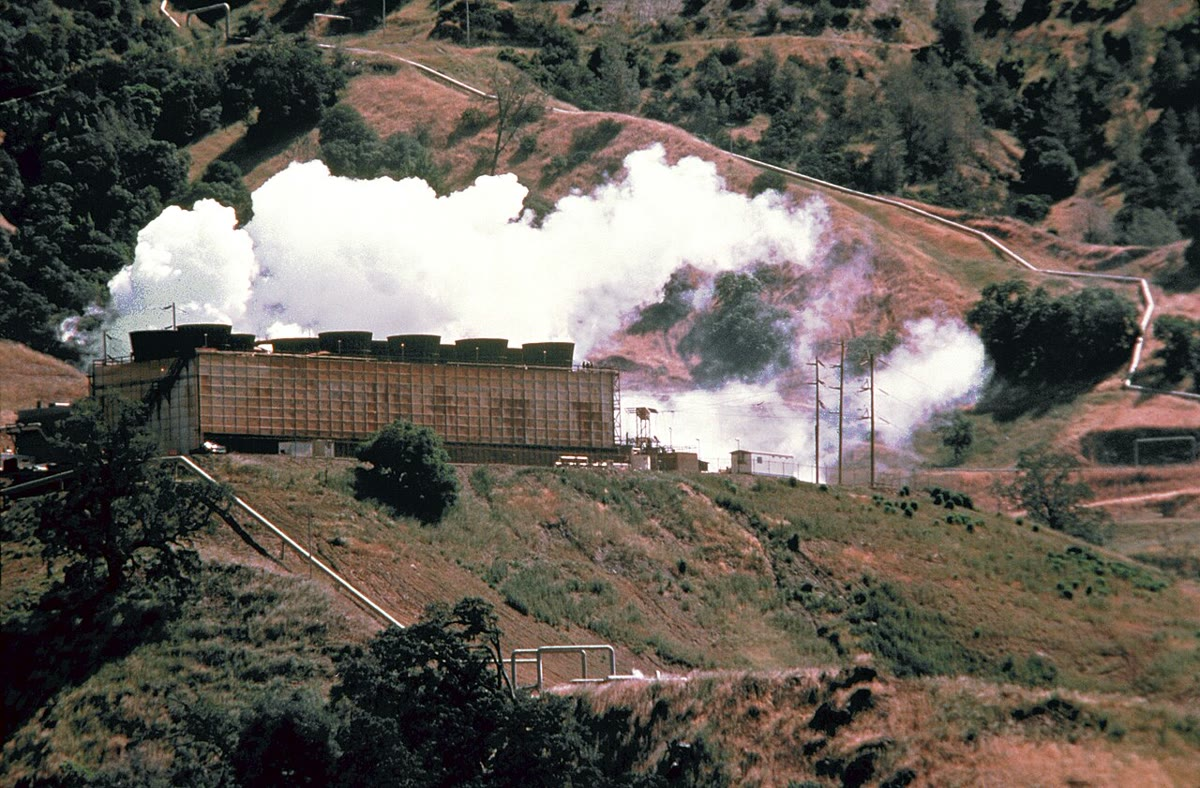
\includegraphics[width=\linewidth]{images/book4/b2-30-geyserville.jpg}
\end{minipage}
\par\smallskip{\small À gauche~: un \omterm{def:b2:energy-geology:geothermal}{système géothermique} à haute enthalpie (schéma, sans échelle)~: l'eau réalimentée sur ses bords (bleu)
est chauffée au-dessus d'une intrusion et remonte par un réservoir fracturé (rouge) jusqu'à une source chaude~; des puits captent le réservoir.
À droite~: une centrale géothermique près de Geyserville, en Californie, en 1982,
avec des conduites de vapeur sur le versant.
Photographie~: U.S. Department of Defense (domaine public).}
\end{omfigure}
% ledger: photo:b2-30-geyserville, usgs08g:egs

\begin{definition}[Sismicité induite]\label{def:b2:energy-geology:induced}
\emph{Sismicité induite}\index{sismicité induite} est une activité sismique causée par des opérations humaines qui modifient la contrainte
ou la pression du fluide interstitiel dans la croûte, le plus souvent
l'injection de fluide dans le sol.
\end{definition}

Le mécanisme est le critère de Coulomb avec pression du fluide interstitiel~: une faille glisse lorsque la contrainte
de cisaillement atteint $\mu(\sigma_n - p)$, si bien qu'augmenter $p$ rapproche de la rupture une faille déjà sollicitée,
sans changer la charge tectonique. Dans les années 1960, des eaux usées injectées dans le socle précambrien fracturé
sous le Rocky Mountain Arsenal, près de Denver, à des profondeurs de 3.7 à
\qty{7.0}{km}, déclenchèrent des séismes~; ceux-ci se confinaient à la partie du réservoir où la
pression avait augmenté de plus de \qty{32}{bar} (\qty{3.2}{MPa}). La forte hausse des séismes
dans l'Oklahoma a été attribuée à l'élimination des eaux usées~: quatre puits à gros débit pourraient expliquer
un cinquième de la sismicité du centre des États-Unis, en déclenchant des séismes à plus de \qty{30}{km} de distance.
Stimuler un réservoir EGS élève la pression
interstitielle de la même façon, par conception.
% ledger: hb81:denver, keranen:oklahoma, usgs08g:egs

\section{Uranium}\label{sec:b2:energy-geology:uranium}

Deux \omterm{def:b2:ore-deposits:types}{types de gisement} illustrent la façon dont l'uranium se concentre~: l'un à une discordance ancienne,
l'autre dans un grès.

\begin{definition}[Gisements d'uranium liés à une discordance et en front d'oxydoréduction]\label{def:b2:energy-geology:uranium}
Un \emph{gisement d'uranium lié à une discordance}\index{gisement d'uranium lié à une discordance} est un corps de pechblende et d'uraninite
remplissant des fractures et des brèches dans des pélites carbonées métamorphisées et dans les arénites quartzeuses
qui les surmontent, sous, au-dessus ou à cheval sur une discordance entre des roches du \omterm{def:b2:precambrian-earth:eons}{Protérozoïque} inférieur et moyen,
dans un \omterm{def:b2:basins-compared:types}{bassin intracratonique}. Un \emph{gisement d'uranium en front d'oxydoréduction}\index{gisement d'uranium en front d'oxydoréduction}
(roll-front) est un corps en forme de croissant de minéraux d'uranium qui recoupe la stratification d'un grès feldspathique
ou tufacé, à la limite entre un terrain oxydé et un terrain réduit, où l'uranium s'est déposé dans un milieu localement
réducteur, parmi la pyrite.
\end{definition}

Les gisements liés à une discordance sont encaissés dans des roches de 1800 à \qty{1200}{\Ma}~: les pélites métamorphisées sous la discordance
et les grès non métamorphisés au-dessus~; leurs roches encaissantes sont chloritisées, et les schistes graphiteux qui accompagnent beaucoup d'entre eux
sont de bons conducteurs électriques, une cible pour les levés électromagnétiques. Key
Lake, Cluff Lake et Rabbit Lake en Saskatchewan, ainsi que Jabiluka et Ranger dans le nord de l'Australie, en sont des exemples.
Les fronts d'oxydoréduction sont plus jeunes, pour la plupart tertiaires~: dans les grès alimentés par des cendres volcaniques felsiques
ou par un granite, les minéraux de fer oxydés se trouvent en amont-pendage du front et les minéraux réduits en aval-pendage,
comme dans les bassins du Wyoming et de la côte du golfe du Texas.
% ledger: b1693:unconformity, b1693:sandstone

\begin{proposition}[Uranium 235 dans le passé]\label{prop:b2:energy-geology:u235}
Soit $r_0$ le rapport atomique actuel $^{235}$U/$^{238}$U et $\lambda_5$, $\lambda_8$ les constantes de désintégration des deux isotopes.
Il y a un temps $t$, ce rapport valait
\begin{equation}
r(t) = r_0\,e^{(\lambda_5 - \lambda_8)\,t} ,
\label{eq:b2:energy-geology:u235}
\end{equation}
et le $^{235}$U formait une fraction $r/(1 + r)$ des atomes d'uranium, en négligeant la trace
de $^{234}$U.
\end{proposition}

\begin{proof}
Tout isotope décroît exponentiellement~: $N_5(\text{actuel}) = N_5(t)\,e^{-\lambda_5 t}$ et $N_8(\text{actuel})
= N_8(t)\,e^{-\lambda_8 t}$. En divisant, $r_0 = r(t)\,e^{-(\lambda_5 - \lambda_8)t}$.
\end{proof}

Avec $\lambda_5 = \qty{9.8485e-10}{an^{-1}}$, $\lambda_8 = \qty{1.55125e-10}{an^{-1}}$ et les abondances actuelles \qty{0.7204}{\percent}
et \qty{99.2742}{\percent}, $r_0 = 0.0072567$~; il y a \qty{2.0}{\Ga}
$r = 0.0381$ et l'uranium naturel contenait \qty{3.67}{\percent} d'$^{235}$U, soit
cinq fois la part actuelle.
% ledger: amherst:constants, iaea:isotopes
% values: r 0.038144, 3.6743 % (calc/ch30.py)

\begin{history}[Un réacteur vieux de deux milliards d'années]
En 1972, des scientifiques français qui mesuraient du minerai d'uranium relevèrent de faibles mais significatifs déficits d'$^{235}$U,
qu'ils rattachèrent à la mine d'Oklo, au Gabon. Là, des poches de roche contenaient jusqu'à \qty{65}{\percent} d'uranium avec une part d'$^{235}$U
aussi faible que la moitié de la part normale, et du néodyme appauvri en son isotope primordial $^{142}$Nd
mais enrichi en isotopes 143 à 150 que produit la fission~:
des réactions en chaîne s'étaient déroulées dans le minerai il y a environ deux milliards d'années,
à environ \qty{300}{bar} et de 400 à \qty{500}{\celsius}. Seize de ces réacteurs naturels sont connus à Oklo et à Bangombé voisin,
les deux seuls gisements au monde où on les a trouvés~; la matière organique avait aidé à concentrer l'uranium,
et l'oxyde d'uranium a retenu sur place, depuis lors, la plupart des actinides
et des produits de fission non volatils.
\end{history}
% ledger: oklo:curtis, oklo:cowan, oklo:gl96, oklo:nagy

\section{Stockage géologique du dioxyde de carbone}\label{sec:b2:energy-geology:ccs}

\begin{definition}[Stockage géologique du \ce{CO2}, mécanismes de piégeage, facteur d'efficacité de stockage]\label{def:b2:energy-geology:ccs}
Le \emph{stockage géologique du \ce{CO2}}\index{stockage géologique du CO$_2$} est l'injection de dioxyde de carbone
dans des formations rocheuses poreuses profondes, des réservoirs de pétrole et de gaz épuisés, des formations salines profondes
ou des couches de charbon, pour une rétention sur de longues durées. Les \emph{mécanismes de piégeage du \ce{CO2}}\index{mécanismes de piégeage du CO$_2$}
qui le retiennent sont le piégeage structural (et stratigraphique) sous une couverture~; le piégeage résiduel, sous forme
d'une phase immobile retenue dans les pores par des forces capillaires~; le piégeage par solubilité, par dissolution dans
l'eau de formation~; le piégeage minéral, par réaction avec des minéraux pour former des carbonates~; et, dans le charbon et
les schistes, l'adsorption sur la matière organique. Le \emph{facteur d'efficacité de stockage}\index{facteur d'efficacité de stockage}
$E$ d'une formation est la fraction de son volume poreux que le
\ce{CO2} injecté peut raisonnablement remplir.
\end{definition}
% ledger: srccs:retention, netl08:saline

Le dioxyde de carbone est un gaz en surface, mais son point critique se situe à \qty{31.0}{\celsius} et
\qty{7.38}{MPa}. Le long d'un géotherme de \qty{25}{\celsius\per\km} partant de \qty{15}{\celsius} sous pression hydrostatique, la température
franchit la valeur critique à \qty{641}{m} et la pression à
\qty{742}{m}~; la masse volumique du \ce{CO2} pur passe de \qty{234}{kg.m^{-3}} à \qty{700}{m} à
\qty{583}{kg.m^{-3}} à \qty{900}{m}, puis se stabilise vers 670 à \qty{700}{kg.m^{-3}} au-dessous de
\qty{1.5}{km}. Une tonne occupe \qty{534}{m^3} en surface et \qty{1.6}{m^3} à \qty{1000}{m},
soit 330 fois moins~; c'est pourquoi les évaluations de stockage ne considèrent que les formations plus profondes que
\qty{800}{m}.
% ledger: nist:co2-critical, data:b4-co2-density, srccs:density, netl08:saline
% values: z_tc 641.2 m, z_pc 742.2 m; volume ratio 331.9 (figdata co2_density.py numbers)

\begin{omfigure}
\centering
\begin{minipage}[b]{0.49\linewidth}\centering
\begin{tikzpicture}
\begin{axis}[omrecord, width=0.95\linewidth, height=5.2cm, xmin=0, xmax=750, ymin=0, ymax=3,
  y dir=reverse, xlabel={masse volumique du \ce{CO2} (\unit{kg.m^{-3}})}, ylabel={profondeur (km)},
  tick label style={font=\scriptsize}, label style={font=\small}]
% computed in figdata/bachelor-2/co2_density.py part profile; ledger: data:b4-co2-density
\addplot[black!45, densely dashed] coordinates {(0,0.742) (750,0.742)};
\node[font=\tiny, text=black!60, anchor=south east] at (axis cs:745,0.73) {pression critique};
\addplot[omDef, line width=1.1pt, mark=*, mark size=0.9pt] table[x=rho, y expr=\thisrow{depth_m}/1000] {figdata/out/bachelor-2-co2_density-profile.dat};
\end{axis}
\end{tikzpicture}
\end{minipage}\hfill
\begin{minipage}[b]{0.49\linewidth}\centering
\begin{tikzpicture}
\begin{axis}[width=0.95\linewidth, height=5.2cm, xmin=0, xmax=4, ymin=0, ymax=100,
  axis x line=bottom, axis y line=left, axis line style={-}, axis on top,
  xlabel={temps après injection (années)}, ylabel={part du \ce{CO2} stocké},
  xtick={0,1,2,3,4}, xticklabels={1,10,100,1000,$10^4$}, ytick=\empty,
  tick label style={font=\scriptsize}, label style={font=\small}]
% schematic, after IPCC SRCCS (2005) Figure 5.9; ledger: srccs:trapping
% bands from the bottom: mineral, solubility, residual, structural (cumulative tops 0/0/1/5/15,
% 2/8/21/40/60, 10/30/56/80/90, 100)
\fill[omLithLime!60!black] (axis cs:0,0) -- (axis cs:1,0) -- (axis cs:2,1) -- (axis cs:3,5) -- (axis cs:4,15) -- (axis cs:4,0) -- cycle;
\fill[omDef!40] (axis cs:0,0) -- (axis cs:1,0) -- (axis cs:2,1) -- (axis cs:3,5) -- (axis cs:4,15) -- (axis cs:4,60) -- (axis cs:3,40) -- (axis cs:2,21) -- (axis cs:1,8) -- (axis cs:0,2) -- cycle;
\fill[omProp!40] (axis cs:0,2) -- (axis cs:1,8) -- (axis cs:2,21) -- (axis cs:3,40) -- (axis cs:4,60) -- (axis cs:4,90) -- (axis cs:3,80) -- (axis cs:2,56) -- (axis cs:1,30) -- (axis cs:0,10) -- cycle;
\fill[black!15] (axis cs:0,10) -- (axis cs:1,30) -- (axis cs:2,56) -- (axis cs:3,80) -- (axis cs:4,90) -- (axis cs:4,100) -- (axis cs:0,100) -- cycle;
\node[font=\scriptsize] at (axis cs:1.1,72) {structurel};
\node[font=\scriptsize] at (axis cs:2.1,38) {résiduel};
\node[font=\scriptsize] at (axis cs:3.1,22) {solubilité};
\node[font=\scriptsize, text=white, anchor=south east] at (axis cs:3.98,0.5) {minéral};
\end{axis}
\end{tikzpicture}
\end{minipage}
\par\smallskip{\small À gauche~: masse volumique du \ce{CO2} pur en fonction de la profondeur, le long d'un géotherme de
\qty{25}{\celsius\per\km} partant de \qty{15}{\celsius}, sous pression hydrostatique. Données~: NIST Chemistry
WebBook (équation d'état de Span--Wagner), dans les conditions du rapport spécial du GIEC
sur la capture et le stockage du dioxyde de carbone (2005). À droite~: comment les mécanismes de piégeage
se partagent le \ce{CO2} stocké au fil du temps (schéma, d'après le même rapport)~: le piégeage par la couverture cède la place aux formes
résiduelle, dissoute et minérale, moins mobiles.}
\end{omfigure}

\begin{proposition}[Capacité de stockage d'une formation]\label{prop:b2:energy-geology:capacity}
Une formation d'aire $A$, d'épaisseur $h$ et de porosité $\phi$, dans laquelle le \ce{CO2} a la masse volumique $\rho$
et de \omterm{def:b2:energy-geology:ccs}{facteur d'efficacité de stockage} $E$, peut stocker la masse
\begin{equation}
M = A\,h\,\phi\,\rho\,E .
\label{eq:b2:energy-geology:capacity}
\end{equation}
Pour un champ pétrolier épuisé ayant produit un volume en surface $N_p$, remplacer l'huile produite
volume pour volume donne $M = \rho\,N_p\,B_o$.
\end{proposition}

\begin{proof}
Le volume poreux vaut $Ah\phi$, dont le \ce{CO2} occupe une fraction $E$, à la masse volumique $\rho$. Dans le
champ pétrolier, l'huile produite occupait $N_pB_o$ dans le réservoir, le volume que prend le \ce{CO2}.
\end{proof}

Pour les formations salines profondes, les simulations donnent un $E$ compris entre 1 et \qty{4}{\percent} du volume poreux
pour un intervalle de confiance de 15 à 85 pour cent, avec une médiane voisine de \qty{2}{\percent}~: l'essentiel de l'espace poreux
n'est jamais atteint, ou garde son eau. Une formation de \qty{1000}{km^2}, de \qty{50}{m} d'épaisseur et de porosité 0.20 à \qty{2000}{m}
($\rho = \qty{686}{kg.m^{-3}}$) stocke \qty{137}{Mt} pour $E =
\qty{2}{\percent}$.
% ledger: netl08:saline, data:b4-co2-density
% values: 1e9*50*0.2*686*0.02 = 1.372e11 kg (calc/ch30.py)

Une fois injecté, le \ce{CO2} remonte sous la couverture et se répand. Derrière le panache qui migre, les forces capillaires
retiennent des saturations résiduelles pouvant atteindre 15 à \qty{25}{\percent} de l'espace poreux~;
la dissolution absorbe de 20 à \qty{60}{kg} de \ce{CO2} par mètre cube d'eau de formation, et dans les formations à écoulement lent,
jusqu'à \qty{30}{\percent} du \ce{CO2} injecté se dissout en quelques dizaines
d'années. Le piégeage par solubilité domine sur des dizaines à des centaines d'années, les formes ioniques sur des centaines
à des milliers d'années, le piégeage minéral sur des milliers à des millions d'années~: les réactions avec les carbonates prennent des jours,
avec les silicates des centaines à des milliers d'années. Le stockage gagne en sûreté en vieillissant, et sur des sites bien choisis et bien gérés,
la rétention de \qty{99}{\percent} ou plus du \ce{CO2} pendant 1000 ans
a été jugée probable.
% ledger: srccs:trapping, srccs:retention

\begin{dated}{2005}
À Sleipner, en mer du Nord à environ \qty{250}{km} de la Norvège, le \ce{CO2} séparé du gaz naturel du champ, soit environ \qty{9}{\percent} de celui-ci,
est injecté depuis octobre 1996 dans la formation d'Utsira, un grès salin non consolidé situé entre 800 et \qty{1000}{m} sous le fond marin,
à raison d'environ \qty{1}{Mt} par an. Au début de 2005, plus de \qty{7}{Mt} avaient été stockées, sur les \qty{20}{Mt}
prévues pour la durée du projet.
Des levés sismiques répétés donnent une image du panache, dont l'emprise était alors d'environ \qty{5}{km^2},
et montrent que la couverture située au-dessus le scelle.
\end{dated}
% ledger: srccs:sleipner

\begin{inthefield}[Lire un puits pendant son forage]
\centering
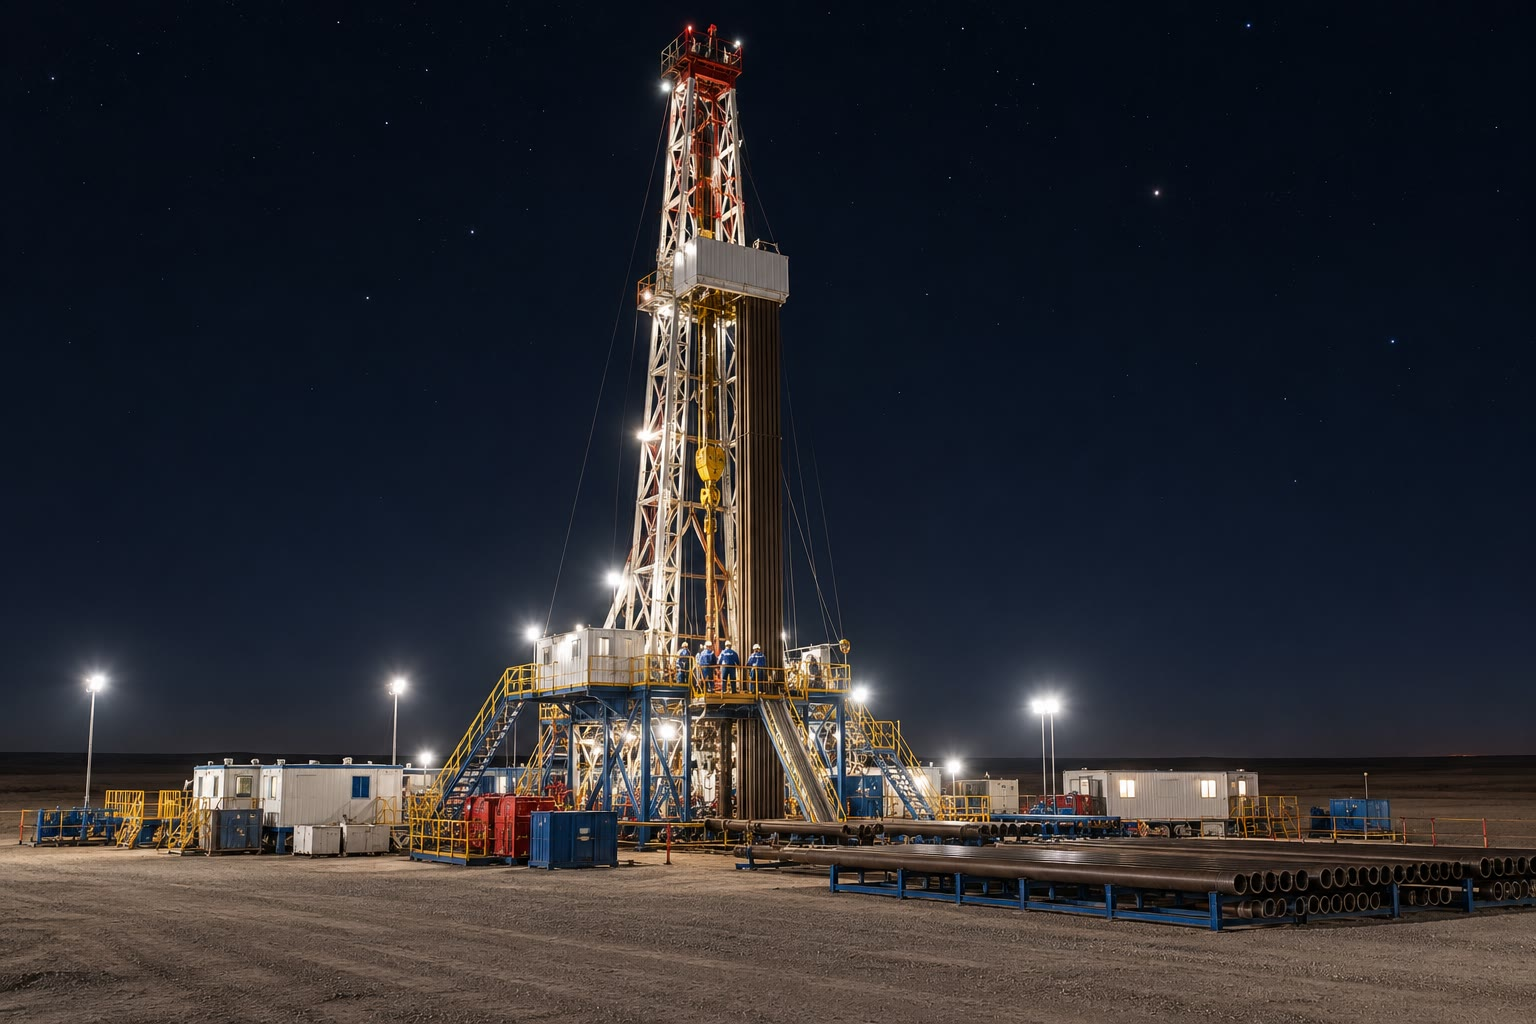
\includegraphics[width=0.56\linewidth]{images/book4/ai/b2-rig-night.jpg}
\par\smallskip{\small Un appareil de forage terrestre de nuit. Illustration générée par IA.}
\par\medskip\raggedright
Lorsqu'une section de puits est achevée, des géophysiciens descendent des outils sur un câble et enregistrent en fonction
de la profondeur les propriétés des roches autour du trou. L'un enregistre leur radioactivité naturelle, faible dans le grès et plus forte dans le schiste~;
un autre enregistre leur masse volumique apparente, à partir de laquelle la porosité se déduit par
(masse volumique des grains $-$ masse volumique apparente)/(masse volumique des grains $-$ masse volumique du fluide), avec \qty{2.65}{g/cm^3} pour
les grains de quartz et environ \qty{1}{g/cm^3} pour l'eau. Lues ensemble, ces diagraphies donnent l'épaisseur
utile du réservoir et la porosité qui entrent dans les formules volumiques de ce chapitre.
\end{inthefield}
% ledger: keys:gamma, keys:density-porosity

\section*{Exercices}\label{sec:b2:energy-geology:exercises}

Données des exercices, sauf indication contraire~: $R = \qty{8.314}{J.mol^{-1}.K^{-1}}$~; un million
d'années vaut \qty{3.156e13}{s}~; kérogène de Green River $A = \qty{9.21e13}{s^{-1}}$, $E/R = \qty{26800}{K}$~;
masses atomiques C 12.011, H 1.008, O 15.999~; masse volumique du \ce{CO2} le long du profil de la figure~:
\qty{1.872}{kg.m^{-3}} en surface, 583 à \qty{900}{m}, 621 à \qty{1000}{m}, 686 à
\qty{2000}{m}. Arrondir à trois chiffres significatifs.
% ledger: codata:R, fp14:gr-daem, data:b4-co2-density

\begin{exercise}[$\star$]\label{exo:b2:energy-geology:1}
(a) Quatre kérogènes immatures ont un H/C atomique de 1.58, 0.95, 1.24 et 1.12. Attribuer à chacun un type et dire
lequel produirait surtout du gaz. (b) Vérifier les rapports H/C et O/C de la formule
C$_{100}$H$_{150}$N$_3$O$_8$S. (c) Les retrouver à partir de la composition massique C \qty{77.4}{\percent}, H
\qty{9.8}{\percent}, O \qty{8.2}{\percent}.
\end{exercise}

\begin{exercise}[$\star$]\label{exo:b2:energy-geology:2}
(a) Cinq échantillons d'une roche mère de type~II ont $R_o$ = 0.45, 0.68, 1.1, 1.6 et \qty{2.5}{\percent}. Décrire l'état de chacun
au regard de l'huile et du gaz. (b) Un kérogène de type~III à $R_o =
\qty{0.68}{\percent}$ produit-il du méthane~? (c) Quelle fraction convertie $F$ d'Easy\%Ro correspond à
$R_o = 0.6$ et \qty{1.3}{\percent}~?
\end{exercise}

\begin{exercise}[$\star$]\label{exo:b2:energy-geology:3}
Un piège couvre \qty{6}{km^2}~; son réservoir a \qty{25}{m} d'épaisseur utile, une porosité de 0.18 et une saturation en eau de 0.30, avec $B_o = 1.25$.
(a) Trouver le volume d'huile dans le réservoir et le STOIIP. (b) Trouver le volume produit
pour des \omterm{def:b2:energy-geology:volumetrics}{taux de récupération} de 0.30 et 0.40.
\end{exercise}

\begin{exercise}[$\star$]\label{exo:b2:energy-geology:4}
Un aquifère gréseux de \qty{200}{m} d'épaisseur sous \qty{10}{km^2} est à \qty{75}{\celsius}. (a) Trouver sa \omterm{def:b2:energy-geology:geothermal}{chaleur en place}
au-dessus de \qty{15}{\celsius}, avec $C = \qty{2.5}{MJ.m^{-3}.K^{-1}}$. (b) À quelle classe d'enthalpie appartient-il~? (c) Trouver la puissance thermique moyenne
sur 30 ans pour $R_g = 0.25$.
\end{exercise}

\begin{exercise}[$\star\star$]\label{exo:b2:energy-geology:5}
(a) Trouver l'énergie d'activation pour laquelle la vitesse d'Arrhenius double entre 100 et
\qty{110}{\celsius}. (b) De combien de fois la vitesse de la réaction de Green River augmente-t-elle sur le même
intervalle~? (c) Laquelle des deux règles accorde le plus de poids au temps passé par une roche à basse température,
et qu'implique-t-elle pour une TTI calculée pour une roche mère de type~I~?
\end{exercise}

\begin{exercise}[$\star\star$]\label{exo:b2:energy-geology:6}
(a) Montrer à partir de \eqref{eq:b2:energy-geology:maturation} que la température de demi-conversion vérifie
$T = (E/R)\big/\ln\bigl[A T^2/(\beta\,(E/R)\ln 2)\bigr]$, et la résoudre par itération
pour le kérogène de Green River chauffé à \qty{1}{\celsius\per\Ma} et à \qty{10}{K} par minute. (b) Comparer
la différence avec l'estimation $(RT^2/E)\ln(\beta_2/\beta_1)$ prise à la plus basse température,
et expliquer le désaccord.
\end{exercise}

\begin{exercise}[$\star\star$]\label{exo:b2:energy-geology:7}
À partir de \eqref{eq:b2:energy-geology:u235} et des données du texte~: (a) trouver la part de $^{235}$U dans l'uranium
naturel il y a \qty{2.0}{\Ga} et \qty{1.8}{\Ga}~; (b) quand cette part valait-elle \qty{3.00}{\percent}~?
(c) Le minerai d'Oklo ne contient que la moitié de la part normale actuelle de $^{235}$U. En négligeant l'$^{238}$U
consommé, quelle fraction du $^{235}$U présent au moment des réactions a été fissionnée, et
pourquoi la décroissance ultérieure ne modifie-t-elle pas la réponse~?
\end{exercise}

\begin{exercise}[$\star\star$]\label{exo:b2:energy-geology:8}
(a) Trouver le volume de \qty{1}{Mt} de \ce{CO2} en surface, à \qty{1000}{m} et à
\qty{2000}{m}. (b) À Sleipner, plus de \qty{7}{Mt} avaient été injectées en 2005, à environ
\qty{900}{m}, dans un panache d'emprise \qty{5}{km^2}. En prenant une porosité de 0.35 et une saturation en \ce{CO2} de 0.30 dans le panache,
trouver le volume de roche qu'il occupe et son épaisseur moyenne.
\end{exercise}

\begin{exercise}[$\star\star$]\label{exo:b2:energy-geology:9}
Un réservoir à haute enthalpie mesure $3 \times 2 \times \qty{1.5}{km}$ à \qty{250}{\celsius}, avec
$C = \qty{2.6}{MJ.m^{-3}.K^{-1}}$. (a) Trouver sa \omterm{def:b2:energy-geology:geothermal}{chaleur en place} au-dessus de \qty{15}{\celsius}. (b) Trouver la
puissance thermique moyenne sur 30 ans pour $R_g = 0.1$ et $0.25$. (c) Son champ couvre \qty{6}{km^2}~;
à raison de 10 à \qty{20}{MW} d'électricité par kilomètre carré, quelle fraction
de la puissance thermique à $R_g = 0.1$ devient de l'électricité~?
\end{exercise}

\begin{exercise}[$\star\star\star$]\label{exo:b2:energy-geology:10}
Une faille à environ \qty{4}{km} porte une contrainte normale de \qty{80}{MPa} et une contrainte de cisaillement de
\qty{22}{MPa}~; son coefficient de frottement vaut 0.6 et la pression interstitielle est hydrostatique,
soit \qty{39}{MPa}. (a) La faille est-elle stable~? Trouver la hausse de pression interstitielle qui la conduit à la rupture, en
mégapascals puis en bars, et la comparer au seuil de Denver. (b) Même question si la contrainte de cisaillement vaut
\qty{24}{MPa}. (c) Expliquer pourquoi des séismes peuvent être déclenchés à des kilomètres d'un puits d'injection,
et des années après le début de l'injection.
\end{exercise}

\begin{exercise}[$\star\star\star$]\label{exo:b2:energy-geology:11}
(a) À partir de l'approximation de \eqref{eq:b2:energy-geology:maturation}, montrer qu'à vitesse de chauffe constante le taux de transformation
passe de \qty{10}{\percent} à \qty{90}{\percent} sur un intervalle de températures
$\Delta T \approx \bigl[\ln\ln 10 - \ln\ln(10/9)\bigr]\,RT^2/E$. (b) Évaluer cet intervalle
pour le kérogène de Green River à \qty{1}{\celsius\per\Ma}. (c) Comparer avec la courbe pleine de la
figure et expliquer la différence.
\end{exercise}

\begin{exercise}[$\star\star\star$]\label{exo:b2:energy-geology:12}
Sleipner doit stocker \qty{20}{Mt} de \ce{CO2}. (a) Trouver le volume d'eau de formation nécessaire pour le dissoudre en totalité, à 20 et à
\qty{60}{kg.m^{-3}}. (b) Trouver son volume en phase libre à
\qty{1000}{m}. (c) Avec $E = \qty{2}{\percent}$, trouver le volume poreux de formation requis, et
l'aire d'une formation de \qty{50}{m} d'épaisseur et de porosité 0.30.
\end{exercise}
% ledger: srccs:trapping, srccs:sleipner, hb81:denver

\begin{problem}[{Problème du week-end --- Un bassin, deux usages}]\label{pb:b2:energy-geology:1}
Dans un bassin fictif, une roche mère de type~I s'est déposée en surface à \qty{120}{\Ma}. Des sédiments se sont ensuite accumulés à \qty{60}{m} par million d'années jusqu'à \qty{70}{\Ma}, puis à \qty{30}{m}
par million d'années depuis. La surface est à \qty{15}{\celsius} et le géotherme est stable à \qty{25}{\celsius\per\km}.
Le kérogène suit la cinétique de Green River du texte, à énergie unique.
Sa cuisine, c'est-à-dire la partie mature de la roche mère, couvre \qty{400}{km^2}, a \qty{50}{m} d'épaisseur
et une masse volumique de \qty{2400}{kg.m^{-3}}, et peut fournir \qty{30}{kg} d'huile par tonne de roche à conversion complète.
L'huile a une masse volumique en surface de \qty{850}{kg.m^{-3}}. Elle remplit un piège de
\qty{12}{km^2} dont le réservoir, centré à \qty{2000}{m}, a une épaisseur utile de \qty{40}{m},
une porosité de 0.22 et une saturation en eau de 0.25, avec $B_o = 1.30$.
Utiliser les données des exercices, et arrondir à
trois chiffres significatifs.

\noindent\textbf{Partie I --- Enfouissement et indice temps--température.}
\begin{enumerate}
  \item Trouver la profondeur et la température de la roche mère à \qty{70}{\Ma} et aujourd'hui.
  \item Trouver sa vitesse de chauffe dans chaque phase.
  \item Trouver le temps passé dans chaque intervalle de \qty{10}{\celsius}, de \qty{15}{\celsius} à
        sa température actuelle.
  \item Calculer sa TTI aujourd'hui (méthode du texte).
  \item Quand, à quelle température et à quelle profondeur a-t-elle atteint une TTI de 15~?
  \item Même question pour 75 et 160.
  \item D'après la TTI, la roche mère génère-t-elle encore de l'huile~?
\end{enumerate}

\noindent\textbf{Partie II --- Conversion par cinétique.}
\begin{enumerate}[resume]
  \item Trouver la constante de vitesse à \qty{90}{\celsius} et montrer que moins de \qty{0.2}{\percent} du
        kérogène a pu être converti avant \qty{70}{\Ma}.
  \item À partir de \eqref{eq:b2:energy-geology:maturation} avec la vitesse de chauffe de la seconde phase,
        trouver la fraction non convertie et le taux de transformation aujourd'hui.
  \item Trouver la température de demi-conversion à cette vitesse de chauffe (exercice~\ref{exo:b2:energy-geology:6}).
  \item Quand a-t-elle été atteinte~?
  \item Comparer avec le moment du maximum de génération donné par la TTI, et expliquer l'écart.
  \item Un kérogène de type~II, d'énergie d'activation moyenne plus faible, se serait-il converti plus tôt ou plus tard~?
\end{enumerate}

\noindent\textbf{Partie III --- Huile générée, en place et récupérable.}
\begin{enumerate}[resume]
  \item Pour un taux de transformation de 0.92, trouver la masse d'huile générée dans la cuisine.
  \item Trouver son volume en surface.
  \item Trouver le STOIIP du piège.
  \item Quelle fraction de l'huile générée le piège retient-il~? Garder \qty{1.56e9}{m^3} pour la question~(15).
  \item Trouver l'huile produite pour un \omterm{def:b2:energy-geology:volumetrics}{taux de récupération} de 0.35.
  \item Pourquoi le \omterm{def:b2:energy-geology:volumetrics}{taux de récupération} est-il bien inférieur à un, et que changerait l'injection de \ce{CO2}~?
\end{enumerate}

\noindent\textbf{Partie IV --- Le champ épuisé comme réservoir de \ce{CO2}.}
\begin{enumerate}[resume]
  \item Trouver la température et la pression hydrostatique du réservoir. Le \ce{CO2} injecté est-il supercritique
        à cet endroit~? Lire sa masse volumique sur la figure.
  \item En gardant $N_p = \qty{2.13e7}{m^3}$, trouver le volume de réservoir libéré par la production.
  \item Exprimer ce volume comme un \omterm{def:b2:energy-geology:ccs}{facteur d'efficacité de stockage} du volume poreux du piège, et comparer avec
        les formations salines.
  \item Une formation saline sous le champ couvre \qty{600}{km^2}, a \qty{80}{m} d'épaisseur, une porosité de
        0.20, avec du \ce{CO2} à \qty{691}{kg.m^{-3}}. Trouver sa capacité pour $E =
        \qty{2}{\percent}$.
  \item En combien d'années d'injection au rythme de Sleipner la remplirait-on~?
  \item Avec $\rho = \qty{686}{kg.m^{-3}}$ et le volume libéré arrondi à \qty{2.77e7}{m^3}, trouver la
        capacité de stockage de \ce{CO2} du réservoir épuisé, en mégatonnes.
\end{enumerate}
\end{problem}
% ledger: fp14:gr-daem, waples80:tti, hamm14:tti-table, netl08:oilgas, netl08:saline, data:b4-co2-density, nist:co2-critical, srccs:sleipner
